%!TEX ROOT=../emnlp2023.tex

% show figures/pipeline.png


\section{Introduction}
\label{sec:introduction}
Lorem ipsum dolor sit amet, consectetur adipiscing elit, sed do eiusmod tempor incididunt ut labore et dolore magna aliqua. Nisl tincidunt eget nullam non. Quis hendrerit dolor magna eget est lorem ipsum dolor sit. Volutpat odio facilisis mauris sit amet massa. Commodo odio aenean sed adipiscing diam donec adipiscing tristique. Mi eget mauris pharetra et. Non tellus orci ac auctor augue. Elit at imperdiet dui accumsan sit. Ornare arcu dui vivamus arcu felis. Egestas integer eget aliquet nibh praesent. In hac habitasse platea dictumst quisque sagittis purus. Pulvinar elementum integer enim neque volutpat ac.

Senectus et netus et malesuada. Nunc pulvinar sapien et ligula ullamcorper malesuada proin. Neque convallis a cras semper auctor. Libero id faucibus nisl tincidunt eget. Leo a diam sollicitudin tempor id. A lacus vestibulum sed arcu non odio euismod lacinia. In tellus integer feugiat scelerisque. Feugiat in fermentum posuere urna nec tincidunt praesent. Porttitor rhoncus dolor purus non enim praesent selementum facilisis. Nisi scelerisque eu ultrices vitae auctor eu augue ut lectus. Ipsum faucibus vitae aliquet nec ullamcorper sit amet risus. Et malesuada fames ac turpis egestas sed. Sit amet nisl suscipit adipiscing bibendum est ultricies. Arcu ac tortor dignissim convallis aenean et tortor at. Pretium viverra suspendisse potenti nullam ac tortor vitae purus. 
\vspace{-1em}
\begin{minipage}{\linewidth}
    \centering
    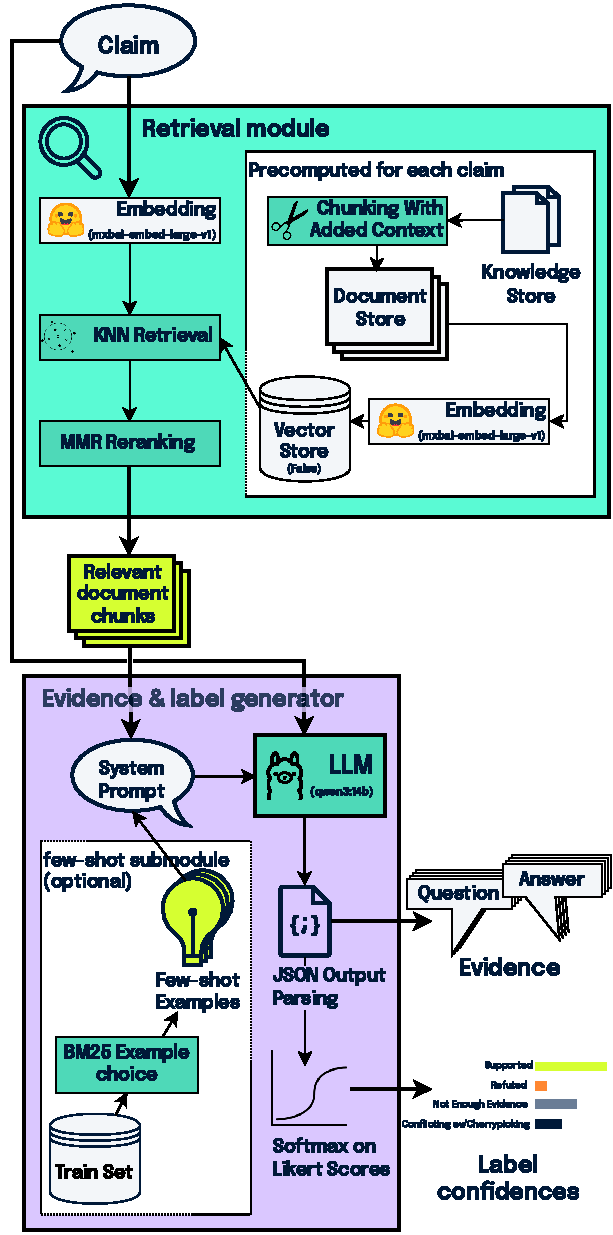
\includegraphics[width=\linewidth]{figures/pipeline.pdf}
    \captionof{figure}{Our refreshed fact-checking pipeline used in CTU AIC FEVER 8 submission, adapted from~\citealt{ullrich-etal-2024-aic}.}
    \label{fig:pipeline}
\end{minipage}
\vspace{1em}

%\section{Related work}
\label{sec:relwork}
\label{avscore}
%\begin{enumerate}
%    \item \textbf{\averitec{} shared task}~\cite{averitec2024} releases the datase of real-world fact-checked claims, annotated with evidence available at the date the claim was made.
%\end{enumerate}

